The von Mises yield criterion suggests that the yielding of materials begins when the second 
deviatoric stress invariant ${\cal I}_2({\bm \tau})$ reaches a critical value. 
For this reason, it is sometimes called the $J_2$-plasticity or $J_2$ flow 
theory\footnote{$J_2$ is the common notation for ${\cal I}_2({\bm \tau})$}. 
It is part of a plasticity theory that applies best to ductile materials, such as metals. 

In material science and engineering the von Mises yield criterion can be also formulated in terms of 
the von Mises stress or equivalent tensile stress, $\sigma_v$, a scalar stress value that can be computed 
from the stress tensor. In this case, a material is said to start yielding when its von Mises stress 
reaches a critical value known as the yield strength, $\sigma_Y$. The von Mises stress is used to predict 
yielding of materials under any loading condition from results of simple uniaxial tensile tests. The 
von Mises stress satisfies the property that two stress states with equal distortion energy have equal 
von Mises stress. 

Because the von Mises yield criterion is independent of the first stress invariant, ${\cal I}_1({\bm \sigma})$, 
it is applicable 
for the analysis of plastic deformation for ductile materials such as metals, as the onset of yield for these materials does not depend on the hydrostatic component of the stress tensor. 

Although formulated by Maxwell in 1865, it is generally attributed to von Mises \cite{vonm13}. 
Huber (1904), in a paper in Polish, anticipated to some extent this criterion. 
Heinrich Hencky formulated the same criterion as von Mises independently in 1924 \cite{henc24,tata03}.
This criterion is also referred to as the Maxwell-Huber-Hencky-von Mises theory. 

The von Mises yield criterion (also known as Prandtl-Reuss yield criterion) is expressed in the principal stresses as
\[
\sigma_v=\sqrt{3J_2'} = \sigma_Y \quad \text{or}, \quad {(\sigma_1 - \sigma_2)^2 + (\sigma_2 - \sigma_3)^2 + (\sigma_3 - \sigma_1)^2 = 2 {\sigma_y}^2 }\!
\]
where $\sigma_Y$ is the yield stress in uniaxial tension.

%Define $k=\sigma_Y/\sqrt{3}$ and 
The von Mises yield criterion writes:

\begin{mdframed}[backgroundcolor=blue!5]
\begin{equation}
F^{VM}= \sqrt{J_2} - \frac{2c}{\sqrt{3}}  \label{vmcrit}
\end{equation}
\end{mdframed}

which is purposely the Drucker-Prager criterion with $\phi=0$.


The following figure shows the von Mises yield surface in the three-dimensional space of principal stresses. 
\begin{center}
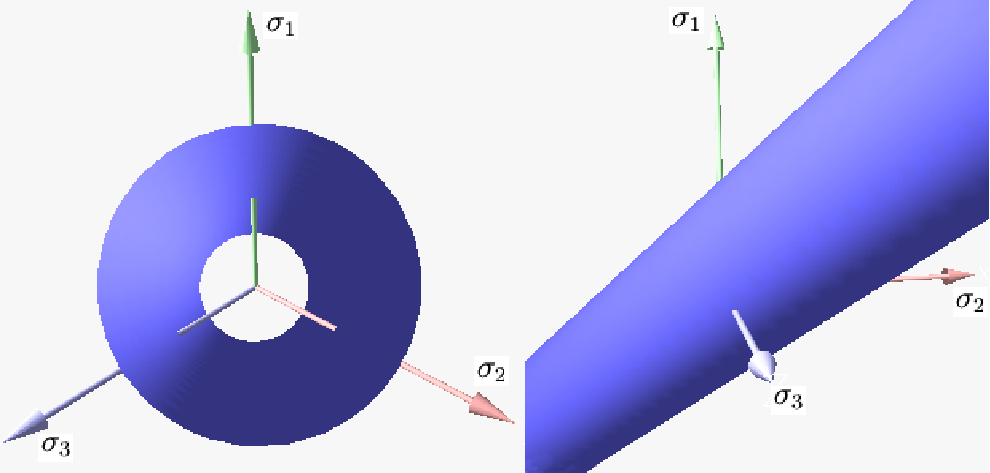
\includegraphics[width=0.6\textwidth]{images/rheology/vonmises/vonmises.pdf}
\end{center}
It is a circular cylinder of infinite length with its axis inclined at equal angles to the three principal stresses. 

\Literature: \cite{papa87,long03}

%\begin{center}
%\includegraphics[width=0.6\textwidth]{RHEOLOGY/viscoplasticity/vMcriterion.pdf}
%\end{center}
